%!TEX root = ../main.tex
\subsubsection{Measurable functions}

We have provide a definition for measurable spaces, but, yes, we still don't know how to measure them. Before that we'll discuss the concept of measurability for functions. The first steps will not involves any kind of function, but we will focus on an easily manageable case. It will be easy to extend those results to the general case.

\begin{defn}
  	Let $(X, \mm)$ be a measurable space, and $(Y, \tau)$ be a topological space. \\
  	We say that $f: X \to Y$ is a \emph{measurable function} if the preimage of any open set is measurable, namely:
  	$$
  		f^{-1}(A) \in \mm 
  		\quad \text{for all } A \in \tau
  	.
  	$$
\end{defn}

Observe that a function defined on two topological spaces, namely $f:(X, \tau_X) \to (Y, \tau_Y)$, if it maps open sets into open sets then it is $\Bc$-measurable with respect to the measurable space $(X, \Bc(X))$. Indeed, for every open set $A \in \tau$, $f^{-1}(A)$ is open in $X$ by definition, and thus $f^{-1}(A) \in \Bc(X)$.

\begin{theo}[Composition of a measurable function with a continuous one]
	Let $f:\; (\Omega, \mm) \to (X, \tau_X)$ be a measurable function and $g:\; (X, \tau_X) \to (Y, \tau_Y)$ be a continuous function.\\
	Then $g \circ f:\; \left(\Omega,\mm \right)\to \left(Y,\tau_Y\right)$ is measurable.
\end{theo}
As we said in the previous remark, $g$ is not only continuous but also $\Bc(X)$-measurable. Here we prove this case, which is more general with respect to the theorem.
\begin{proof}
	Let $A \subset Y$ be an open set, then $g^{-1}\left(A\right)\in \Bc\left(X\right)$. Now let $B \subset X$ be open, and $f^{-1}(B) \in \mm$.
	
	As $\Bc(X)$ is generated by all the open sets in $X$ and is closed with respect to union and complement, $f^{-1}(g^{-1}(A)) \in \mm$ and this means that $g\circ f$ is $\mm$-measurable (in case $A = \varnothing$ we have $g\circ f (A) = \varnothing \in \mm$) .
\end{proof}

If $f$ and $g$ are just measurable, then $g \circ f$ is not necessarily measurable, even if $f$ is continuous.

\paragraph{Measurable functions in $\RR$}There are some important results that holds when working in $\RR$. First, the previous theorem can be extended to the multi dimensional case.
\begin{theo}\label{multiple-measurable-function-composed-contiunuous} 
	Let $\left(u,v\right) : \left(\Omega,\mm\right)\to\RR^2$ be $\mm$-measurable. \\
	Moreover, let $\Phi : \ \RR^2 \to \left(X,\tau \right)$ be continuous.
	
	Then $h=\Phi\left(u,v\right):\ \left(\Omega,\mm\right)\to \left(X,\tau\right)$ is $\mm$-measurable.
\end{theo}
\begin{proof}
	Let $A \subseteq X$ be open. Then $\Phi^{-1}(A)\subseteq \RR^2$ is open. \\
	Thanks to theorem \vref{open-set-RR-intervals}, we have that $\Phi^{-1}(A) = \bigcup_{i \in \NN} I_{i}\times J_{i}$ where $I_{i},\ J_{i} \subset \RR$ are intervals. \\
	Finally, observe that $h^{-1}\left(I_{i}\times J_{i}\right)=u^{-1}\left(I_{i}\right)\cap v^{-1}\left(J_{i}\right) \in \mm$.
\end{proof} 
This theorem has several implications: if $u,v:\left(\Omega,\mm\right)\to\RR^2$ are measurable, than $u\pm v$, $uv$, $|u|$, $u^+$, $u_-$ and other elementary operation with these functions returns $\mm$-measurable functions.

The following proposition shows a topological property of the set $\RR$, it will turn useful in many fields.

\begin{theo} \label{open-set-RR-intervals}
	Every open set $\Omega \in \RR$ can be written in a unique way as countable union of mutually disjoint intervals, namely: $$\Omega = \bigcup_{j=1}^{\infty} I_j \qquad I_j=\left(a_j,b_j\right).$$
	
	Every open set $\Omega \in \RR^N$, with $n>1$, can be written in a unique way as countable union of $n$ intervals,namely:
	$$\Omega = \bigcup_{j=1}^{\infty} I_j \qquad I_j=\left(a_j^1,b_j^1\right)\times\left(a_j^2,b_j^2\right)\times\cdots\times\left(a_j^n,b_j^n\right).$$
\end{theo}
\begin{proof}
	\textit{Step 1. The intervals are well defined}:\\
	First, consider $x \in \Omega$: we need to build the largest open interval $I_x\subset \Omega$ containing $x$.\\
	We define $I_x = (a_x,b_x)$ where:
	$$ 
		a_x 
		\coloneqq \inf \{a < x: (a,x) \subset \Omega \} \ 
		\text{ and } \ b_x \coloneqq \sup \{b>x:(x,b) \subset \Omega \}
	;
	$$
	notice that $I_x \neq \varnothing$, $a_x \neq x$  and $b_x \neq x$ since $\Omega$ is open and $x \in \Omega$.\\
	Certainly we have that $a_x \in [-\infty, x)$ and $b_x \in (x, +\infty]$.\\
	Moreover, we show that $I_x \in \Omega$; let $w \in I_x$, without loss of generality we assume that $x < w < b_x$. Then by the definition of $b_x$, it exists $b > w$ such that $(x,b) \in \Omega$: then $w \in \Omega$.
	
	\textit{Step 2. The set is the union of the intervals}:\\
	Consider the collection of open intervals $\{I_x\}_{x\in \Omega}$. Since each $x\in \Omega$ and $x \in i_x \subseteq \Omega$, then 
	$$
		\Omega 
		= \bigcup_{x\in \Omega} I_x
	.
	$$
	Here we have two problems: first, the family $\{I_x\}_{x\in \Omega}$ may not be disjoint; second the same family can be uncountable.
	
	\textit{Step 3. The family of intervals is disjoint}:\\
	To solve the first problem we have to prove that if $x,y \in \Omega$, then either $I_x = I_y$ or $I_x \cap I_y = \varnothing$.\\
	If $I_x \cap I_y \neq \varnothing$ then $I_x \cup I_y$ is still an open interval, and it contains both $x$ and $y$, and it is a subset of $\Omega$.\\
	Since $I_x$, as we proved before, is the largest open interval in $\Omega$ containing $x$, we have:
	$$
		I_x \supseteq I_x \cap I_y \supseteq I_x 
		\implies I_x = I_x \cup I_y
	.
	$$
	Similarly we can show that $I_x = I_y$.
	
	\textit{Step 4. The family of intervals is countable}:\\
	Since for any $x\in \Omega$ there exists a rational number $q \in I_x \subseteq \Omega$, and we have that $I_x \cap I_q \neq \varnothing$, hence $I_x = I_q$.\\
	This means that: $$\Omega = \bigcup_{x\in\Omega} I_x = \bigcup_{q \in \QQ \cap \Omega} I_q$$
	as $\QQ$ is countable, then $\Omega \cap \QQ$ is countable as well, hence the thesis.	
\end{proof}
This proof can be extended to $\RR^N$ case.

\begin{prop}
	Every open set $\Omega \subset \RR^N$ can be written as a countable union of closed, disjoint cubes, namely:
	$$ \Omega = \bigcup_{j = 1}^{\infty} R_j$$
	where
	$$R_j = [a_j^1,b_j^1]\times[a_j^2,b_j^2]\times\cdots\times[a_j^n,b_j^n]$$
	with
	$$a_j^i < b_j ^i \ \forall i \text{ and } \mathring R_i \cap \mathring R_k = \varnothing \ k \neq i.$$ 
\end{prop}
Observe that $R_j$ must be almost disjoints.


This last results is about the Borel $\sigma$-algebras of $\RR$ and $\RR^\star$; they don't need the entire topology to be generated. 
\begin{theo}\label{borel-sigma-algebra-of-rr}
	The Borel $\sigma$-algebra of $\RR$ and $\RR^\star$ are defined as follows:
	$$\Bc(\RR)=\sca{\{\left(a,b\right)\}_{a,b \in \RR}} \qquad \Bc(\RR^\star )=\sca{\{\left(a,+\infty\right]\}_{a\in\RR}}.$$
\end{theo}
\begin{proof}
	\textit{Proof of the generator sets of $\Bc(\RR)$}:\\
	This first statement follows from theorem \vref{open-set-RR-intervals}.
	
	\textit{Proof of the generator sets of $\Bc(\RR^\star)$}:\\
	For the second one, let us consider the set $\left(a, +\infty\right]$, which is open $\forall a \in \RR$. So we have that:
	$$\Bc(\RR^\star) \supseteq \sca{\{\left(a,+\infty\right]_{a \in \RR}\}} \eqqcolon \mm.$$
	Now we want to prove that $\Bc(\RR^\star) \subseteq \mm$, by checking that the sets $[-\infty, a]$, $(a, b)$, $(b, +\infty]$ are contained in $\mm$ for all $a$, $b$:
	\begin{align*}
	[-\infty, a] &= (a, +\infty]\comp \in \mm \\
	\left[-\infty,a\right) &= \bigcup_{n=1}^\infty \left(-\infty, a - \frac 1 n \right] \in \mm \\
	(a,b) &= \left[-\infty,b\right) \cap \left(a,+\infty\right] \in \mm
	\end{align*}
	The sets $[-\infty, a]$, $(a, b)$, $(b, +\infty]$ form a base for the topology of $\RR^\star$, and thus $\mm \supseteq \Bc(\RR^\star)$.\\
	That proves that $\Bc(\RR^\star) \subseteq \mm$.
\end{proof}


Indeed, those structures are generated as follows: 
	$$\Bc(\RR)=\sca{\{\left(a,b\right)\}_{a,b \in \RR}} \qquad \Bc(\RR^\star )=\sca{\{\left(a,+\infty\right]\}_{a\in\RR}}$$
See proposition \vref{borel-sigma-algebra-of-rr} for the proof of this result.


\paragraph{Measurability for sequence of functions} Now we pose the following problem: having a sequence of measurable function which converges to a limit function, is that function measurable? Before look at these results, recall the notions of \textit{liminf} and \textit{limsup} explained in the appendix.

\begin{theo} \label{lim-are-measurable}
	Let $f_n:\left(\Omega,\mm\right)\to \RR^\star$ be $\mm$-measurable functions for all $n \in \NN$. \\
	Then $\sup f_n$, $\inf f_n$, $\limsup f_n$,  $\liminf f_n$ are all $\mm$-measurable.
\end{theo}
\begin{proof}
	\textit{Step 1. Inferior and superior}:\\ Consider $g(x) \coloneqq \sup f_n(x)$:
	\begin{align*}
	g^{-1}((a, +\infty])
	& = \{ x \in \RR^\star \ |\ \sup f_n(x) > a \}\\
	& = \{ x \in \RR^\star \ |\ \exists \, n : f_n(x) > a \} \\
	& = \{ x \in \RR^\star \ |\ \exists \, n : x \in f_n^{-1}((a, +\infty]) \} \\
	& = \bigcup_{n\in\NN}f_n^{-1}\left(\left(a,+\infty\right]\right)\\
	& \in\mm
	.
	\end{align*}

	We need to prove the measurability only on $(a, +\infty]$, the remaining comes by properties of $\sigma$-algebra and topology; indeed, all the generators of the topology $\tau_C^\star$ have a counterimage in $\mm$.
	
	Consider now $g(x) \coloneqq \inf f_n(x)$. Arguing as before we get: $g^{-1}\left(\left[-\infty,a\right)\right) = \bigcup_{n\in\NN}f_n^{-1}\left(\left[-\infty,a\right)\right)\in\mm$.
	
	\textit{Step 2. Liminf and limsup}:\\
	Then consider $g(x) \coloneqq \limsup f_n(x) = \inf_{n\ge 0}\left(\sup_{k\geq n} f_k(x) \right)$.
	In the previous lines we have shown that $\sup_{k \geq 0} f_k$ is measurable, and so is the function $h_n = \sup_{k \geq n} f_k$, for any $n \in \NN$; the infimum of such sequence, which is $\inf h_n \left(\sup_{k \geq n} f_k\right) = g(x)$, is also measurable as we shown before.
	
	We can argue in a similar way for $\liminf f_n(x)$ and conclude the proof.
\end{proof}

\paragraph{Simple functions} Let consider a simple kind of functions for which is easy to find a measure. Those function will be the prototype of functions in general and though them we will extend their measure to all the measurable functions.

\begin{defn}\label{simple-function}
	Let $\left(\Omega,\mm\right)$ be a measurable space $\left(\Omega \neq \varnothing\right)$.\\
	We say that $s:\Omega \to \RR$ is a \emph{simple function} if it has the following form: $$s(t)=\sum_{n=1}^N a_n\Ind_{E_n}(t)$$
	where $a_j \in \RR$ and $\{E_j\}_{j=1}^N$ is a partition of $\Omega$ made of measurable sets.
\end{defn}

The set function $\Ind_{E}$ the indicator function.

\begin{exam}\label{ex:simple-functions}
	The function: $s(t)=\Ind_{[-\infty,2)}(t)+3\Ind_{[2,3]}(t)-\Ind_{(3,+\infty)}(t)$ is a simple function.
\end{exam}

\begin{figure}[htpb]
	\centering
	\tikzset{every picture/.style={line width=0.75pt}} %set default line width to 0.75pt        

	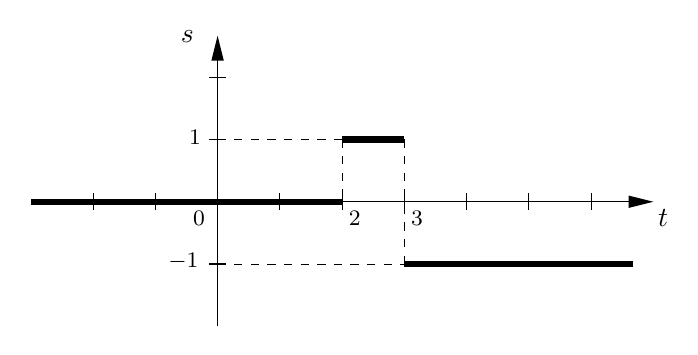
\begin{tikzpicture}[x=0.75pt,y=0.75pt,yscale=-1,xscale=1]
	\draw (80,90) -- (378,90) (110,86) -- (110,94)(140,86) -- (140,94)(170,86) -- (170,94)(200,86) -- (200,94)(230,86) -- (230,94)(260,86) -- (260,94)(290,86) -- (290,94)(320,86) -- (320,94)(350,86) -- (350,94) ;
	\draw [shift={(380,90)}, rotate = 180] [fill={rgb, 255:red, 0; green, 0; blue, 0 }  ][line width=0.08]  [draw opacity=0] (12,-3) -- (0,0) -- (12,3) -- cycle    ;
	\draw (170,150) -- (170,12) (166,120) -- (174,120)(166,90) -- (174,90)(166,60) -- (174,60)(166,30) -- (174,30) ;
	\draw [shift={(170,10)}, rotate = 90] [fill={rgb, 255:red, 0; green, 0; blue, 0 }  ][line width=0.08]  [draw opacity=0] (12,-3) -- (0,0) -- (12,3) -- cycle    ;
	\draw [line width=2.25]    (80,90) -- (230,90) ;
	\draw [dashed, very thin]  (230,60) -- (230,90) ;
	\draw [line width=2.25]    (230,60) -- (260,60) ;
	\draw [line width=2.25]    (260,120) -- (370,120) ;
	\draw [dashed, very thin]  (260,60) -- (260,120) ;
	\draw [dashed, very thin]  (170,60) -- (230,60) ;
	\draw [dashed, very thin]  (170,120) -- (260,120) ;

	\draw (157,93.4) node [anchor=north west][inner sep=0.75pt]  [font=\footnotesize]  {$0$};
	\draw (232,93.4) node [anchor=north west][inner sep=0.75pt]  [font=\footnotesize]  {$2$};
	\draw (155,54.4) node [anchor=north west][inner sep=0.75pt]  [font=\footnotesize]  {$1$};
	\draw (262,93.4) node [anchor=north west][inner sep=0.75pt]  [font=\footnotesize]  {$3$};
	\draw (145,113.4) node [anchor=north west][inner sep=0.75pt]  [font=\footnotesize]  {$-1$};
	\draw (151,6.4) node [anchor=north west][inner sep=0.75pt]  [font=\normalsize]  {$s$};
	\draw (381,92.4) node [anchor=north west][inner sep=0.75pt]  [font=\normalsize]  {$t$};
	\end{tikzpicture}
	\caption{Plot of the function of example \vref{ex:simple-functions}.}
\end{figure}
\FloatBarrier

\begin{theo}
	Let $(\Omega,\mm)$ be a measurable space, with $\Omega \neq \varnothing$.\\
	For any function $f:(\Omega,\mm) \to \left[0,+\infty\right]$, $\mm$-measurable, there exists a sequence of simple functions 
	$$
		\{s_n\}_{n\in \NN}: 
		\ (\Omega,\mm)\to\left[0,+\infty\right]
	$$
	such that:
	\begin{itemize}
		\item the sequence is monotone: 
			$$
				s_n(t) \leq s_{n+1}(t)
				\quad \forall t\in \Omega 
				\quad \forall n\in\NN
			;
			$$
		\item the sequence is dominated: 
			$$
				0 \leq s_n(t) \leq f(t)
				\quad \forall t \in \Omega 
				\quad \forall n\in\NN
			;
			$$
		\item the sequence converges point-wise: 
			$$
				\lim\limits_{n \to + \infty} s_n(t) = f(t) 
				\quad \forall t\in \Omega
			.
			$$
	\end{itemize}
	Moreover, if the function is bounded, namely there exists $M>0$ such that $f(t) < M$ for any $t \in \Omega$, the sequence converges uniformly to $f$ in $\Omega$.
\end{theo}

Notice that $[0,+\infty]$ is a topological space with the topology inducted by $(\RR^\star, \tau_C^\star)$.

The following is a constructive proof in which the sequence object of the theorem is built.

\begin{proof}
	Let $n \in \NN_0$, split $\left[0,n\right)$ in $k=n2^n$ intervals $\left[a_j,b_j\right)$ of length $2^{-n}$.
	
	Take $E_0=f^{-1}(\left[n,+\infty\right])$ and $E_j=f^{-1}([a_j,b_j])$, which are $\mm$-measurable.\\
	%\missingfigure{$E_j=f^{-1}([a_j,b_j])$}
	\begin{figure}[htpb]
		\centering
		\tikzset{every picture/.style={line width=0.75pt}} %set default line width to 0.75pt        

		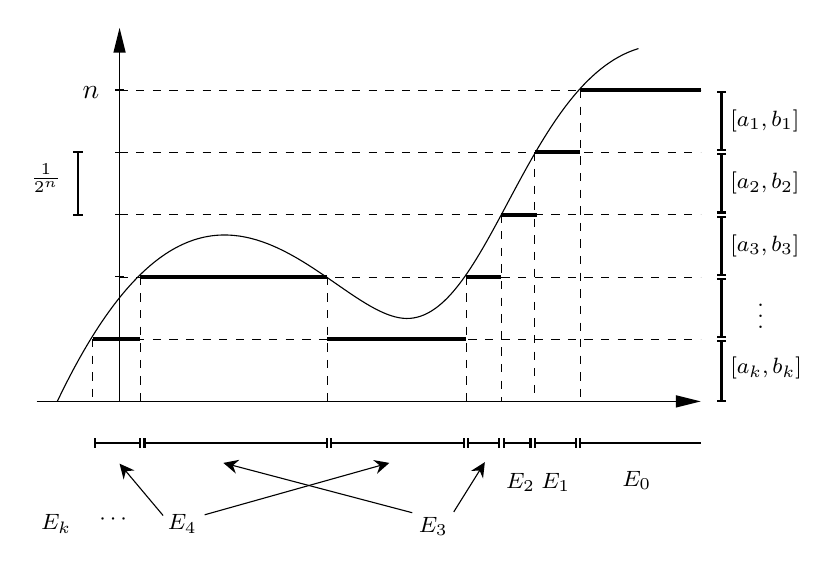
\begin{tikzpicture}[x=0.75pt,y=0.75pt,yscale=-1,xscale=1]
		%uncomment if require: \path (0,303); %set diagram left start at 0, and has height of 303

		\draw    (130,210) .. controls (204,55) and (262,173) .. (300,170) .. controls (338,167) and (357,56) .. (410,40) ;
		\draw [line width=0.75]  [dashed, very thin]  (160,60) -- (440,60) ;
		\draw [line width=0.75]  [dashed, very thin]  (160,90) -- (440,90) ;
		\draw [line width=0.75]  [dashed, very thin]  (160,120) -- (440,120) ;
		\draw  [dashed, very thin]  (160,150) -- (440,150) ;
		\draw  [dashed, very thin]  (160,180) -- (440,180) ;
		\draw  [dashed, very thin]  (170,150) -- (170,210) ;
		\draw  [dashed, very thin]  (260,150) -- (260,210) ;
		\draw  [dashed, very thin]  (327,150) -- (327,210) ;
		\draw  [dashed, very thin]  (344,120) -- (344,210) ;
		\draw  [dashed, very thin]  (360,90) -- (360,210) ;
		\draw  [dashed, very thin]  (382,60) -- (382,210) ;
		\draw  [dashed, very thin]  (147,180) -- (147,210) ;
		\draw [line width=1.5]    (147,180) -- (170,180) ;
		\draw [line width=1.5]    (170,150) -- (260,150) ;
		\draw [line width=1.5]    (327,150) -- (344,150) ;
		\draw [line width=1.5]    (344,120) -- (361,120) ;
		\draw [line width=1.5]    (360,90) -- (382,90) ;
		\draw [line width=1.5]    (382,60) -- (440,60) ;
		\draw [line width=1.5]    (260,180) -- (327,180) ;
		\draw [line width=0.75]    (382,230) -- (440,230) ;
		\draw [shift={(382,230)}, rotate = 180] [color={rgb, 255:red, 0; green, 0; blue, 0 }  ][line width=0.75]    (0,2.24) -- (0,-2.24)   ;
		\draw [line width=0.75]    (360,230) -- (380,230) ;
		\draw [shift={(380,230)}, rotate = 180] [color={rgb, 255:red, 0; green, 0; blue, 0 }  ][line width=0.75]    (0,2.24) -- (0,-2.24)   ;
		\draw [shift={(360,230)}, rotate = 180] [color={rgb, 255:red, 0; green, 0; blue, 0 }  ][line width=0.75]    (0,2.24) -- (0,-2.24)   ;
		\draw [line width=0.75]    (345,230) -- (358,230) ;
		\draw [shift={(358,230)}, rotate = 180] [color={rgb, 255:red, 0; green, 0; blue, 0 }  ][line width=0.75]    (0,2.24) -- (0,-2.24)   ;
		\draw [shift={(345,230)}, rotate = 180] [color={rgb, 255:red, 0; green, 0; blue, 0 }  ][line width=0.75]    (0,2.24) -- (0,-2.24)   ;
		\draw [line width=0.75]    (328,230) -- (343,230) ;
		\draw [shift={(343,230)}, rotate = 180] [color={rgb, 255:red, 0; green, 0; blue, 0 }  ][line width=0.75]    (0,2.24) -- (0,-2.24)   ;
		\draw [shift={(328,230)}, rotate = 180] [color={rgb, 255:red, 0; green, 0; blue, 0 }  ][line width=0.75]    (0,2.24) -- (0,-2.24)   ;
		\draw [line width=0.75]    (172,230) -- (260,230) ;
		\draw [shift={(260,230)}, rotate = 180] [color={rgb, 255:red, 0; green, 0; blue, 0 }  ][line width=0.75]    (0,2.24) -- (0,-2.24)   ;
		\draw [shift={(172,230)}, rotate = 180] [color={rgb, 255:red, 0; green, 0; blue, 0 }  ][line width=0.75]    (0,2.24) -- (0,-2.24)   ;
		\draw [line width=0.75]    (262,230) -- (326,230) ;
		\draw [shift={(326,230)}, rotate = 180] [color={rgb, 255:red, 0; green, 0; blue, 0 }  ][line width=0.75]    (0,2.24) -- (0,-2.24)   ;
		\draw [shift={(262,230)}, rotate = 180] [color={rgb, 255:red, 0; green, 0; blue, 0 }  ][line width=0.75]    (0,2.24) -- (0,-2.24)   ;
		\draw [line width=0.75]    (148,230) -- (170,230) ;
		\draw [shift={(170,230)}, rotate = 180] [color={rgb, 255:red, 0; green, 0; blue, 0 }  ][line width=0.75]    (0,2.24) -- (0,-2.24)   ;
		\draw [shift={(148,230)}, rotate = 180] [color={rgb, 255:red, 0; green, 0; blue, 0 }  ][line width=0.75]    (0,2.24) -- (0,-2.24)   ;
		\draw [line width=0.75]    (450,61) -- (450,89) ;
		\draw [shift={(450,89)}, rotate = 270] [color={rgb, 255:red, 0; green, 0; blue, 0 }  ][line width=0.75]    (0,2.24) -- (0,-2.24)   ;
		\draw [shift={(450,61)}, rotate = 270] [color={rgb, 255:red, 0; green, 0; blue, 0 }  ][line width=0.75]    (0,2.24) -- (0,-2.24)   ;
		\draw [line width=0.75]    (450,91) -- (450,119) ;
		\draw [shift={(450,119)}, rotate = 270] [color={rgb, 255:red, 0; green, 0; blue, 0 }  ][line width=0.75]    (0,2.24) -- (0,-2.24)   ;
		\draw [shift={(450,91)}, rotate = 270] [color={rgb, 255:red, 0; green, 0; blue, 0 }  ][line width=0.75]    (0,2.24) -- (0,-2.24)   ;
		\draw [line width=0.75]    (450,121) -- (450,149) ;
		\draw [shift={(450,149)}, rotate = 270] [color={rgb, 255:red, 0; green, 0; blue, 0 }  ][line width=0.75]    (0,2.24) -- (0,-2.24)   ;
		\draw [shift={(450,121)}, rotate = 270] [color={rgb, 255:red, 0; green, 0; blue, 0 }  ][line width=0.75]    (0,2.24) -- (0,-2.24)   ;
		\draw [line width=0.75]    (450,151) -- (450,179) ;
		\draw [shift={(450,179)}, rotate = 270] [color={rgb, 255:red, 0; green, 0; blue, 0 }  ][line width=0.75]    (0,2.24) -- (0,-2.24)   ;
		\draw [shift={(450,151)}, rotate = 270] [color={rgb, 255:red, 0; green, 0; blue, 0 }  ][line width=0.75]    (0,2.24) -- (0,-2.24)   ;
		\draw [line width=0.75]    (450,181) -- (450,210) ;
		\draw [shift={(450,210)}, rotate = 270] [color={rgb, 255:red, 0; green, 0; blue, 0 }  ][line width=0.75]    (0,2.24) -- (0,-2.24)   ;
		\draw [shift={(450,181)}, rotate = 270] [color={rgb, 255:red, 0; green, 0; blue, 0 }  ][line width=0.75]    (0,2.24) -- (0,-2.24)   ;
		\draw [line width=0.75]    (140,90) -- (140,120) ;
		\draw [shift={(140,120)}, rotate = 270] [color={rgb, 255:red, 0; green, 0; blue, 0 }  ][line width=0.75]    (0,2.24) -- (0,-2.24)   ;
		\draw [shift={(140,90)}, rotate = 270] [color={rgb, 255:red, 0; green, 0; blue, 0 }  ][line width=0.75]    (0,2.24) -- (0,-2.24)   ;
		\draw    (181,265) -- (161.93,242.3) ;
		\draw [shift={(160,240)}, rotate = 49.97] [fill={rgb, 255:red, 0; green, 0; blue, 0 }  ][line width=0.08]  [draw opacity=0] (7.14,-3.43) -- (0,0) -- (7.14,3.43) -- (4.74,0) -- cycle    ;
		\draw    (201,264.64) -- (287.11,240.45) ;
		\draw [shift={(290,239.64)}, rotate = 164.31] [fill={rgb, 255:red, 0; green, 0; blue, 0 }  ][line width=0.08]  [draw opacity=0] (7.14,-3.43) -- (0,0) -- (7.14,3.43) -- (4.74,0) -- cycle    ;
		\draw    (301,263.64) -- (212.9,240.41) ;
		\draw [shift={(210,239.64)}, rotate = 14.77] [fill={rgb, 255:red, 0; green, 0; blue, 0 }  ][line width=0.08]  [draw opacity=0] (7.14,-3.43) -- (0,0) -- (7.14,3.43) -- (4.74,0) -- cycle    ;
		\draw    (321,263.28) -- (334.41,241.83) ;
		\draw [shift={(336,239.28)}, rotate = 122.01] [fill={rgb, 255:red, 0; green, 0; blue, 0 }  ][line width=0.08]  [draw opacity=0] (7.14,-3.43) -- (0,0) -- (7.14,3.43) -- (4.74,0) -- cycle    ;
		\draw    (160,210) -- (160,32) (158,180) -- (162,180)(158,150) -- (162,150)(158,120) -- (162,120)(158,90) -- (162,90)(158,60) -- (162,60) ;
		\draw [shift={(160,30)}, rotate = 90] [fill={rgb, 255:red, 0; green, 0; blue, 0 }  ][line width=0.08]  [draw opacity=0] (12,-3) -- (0,0) -- (12,3) -- cycle    ;
		\draw    (120,210) -- (438,210) ;
		\draw [shift={(440,210)}, rotate = 180] [fill={rgb, 255:red, 0; green, 0; blue, 0 }  ][line width=0.08]  [draw opacity=0] (12,-3) -- (0,0) -- (12,3) -- cycle    ;

		\draw (116,94.4) node [anchor=north west][inner sep=0.75pt]  [font=\footnotesize]  {$\frac{1}{2^{n}}$};
		\draw (141,57) node [anchor=north west][inner sep=0.75pt]    {$n$};
		\draw (401,242.4) node [anchor=north west][inner sep=0.75pt]  [font=\footnotesize]  {$E_{0}$};
		\draw (362,243.4) node [anchor=north west][inner sep=0.75pt]  [font=\footnotesize]  {$E_{1}$};
		\draw (345,243.4) node [anchor=north west][inner sep=0.75pt]  [font=\footnotesize]  {$E_{2}$};
		\draw (303,264.4) node [anchor=north west][inner sep=0.75pt]  [font=\footnotesize]  {$E_{3}$};
		\draw (182,263.4) node [anchor=north west][inner sep=0.75pt]  [font=\footnotesize]  {$E_{4}$};
		\draw (453,68.4) node [anchor=north west][inner sep=0.75pt]  [font=\footnotesize]  {$[ a_{1} ,b_{1}]$};
		\draw (453,187.4) node [anchor=north west][inner sep=0.75pt]  [font=\footnotesize]  {$[ a_{k} ,b_{k}]$};
		\draw (453,98.4) node [anchor=north west][inner sep=0.75pt]  [font=\footnotesize]  {$[ a_{2} ,b_{2}]$};
		\draw (453,128.4) node [anchor=north west][inner sep=0.75pt]  [font=\footnotesize]  {$[ a_{3} ,b_{3}]$};
		\draw (466,153.73) node [anchor=north west][inner sep=0.75pt]  [font=\footnotesize]  {$\vdots $};
		\draw (121,263.4) node [anchor=north west][inner sep=0.75pt]  [font=\footnotesize]  {$E_{k}$};
		\draw (149,263.4) node [anchor=north west][inner sep=0.75pt]  [font=\footnotesize]  {$\cdots $};

		\end{tikzpicture}
		\caption{Construction of approximating simple functions.}
	\end{figure}
	\FloatBarrier
	Define now: 
		$$
			s_n(t)
			\coloneqq n\Ind_{E_0}(t)
			+\sum_{j=1}^{n2^n}a_j \Ind_{E_j}(t)
		.
		$$
	By definition $s_n(t)$ is a simple function for any $n \in \NN$, with $s_n(t) = a_j$ if $f(t) \in [a_j, b_j)$, and $s_n(t) = n$ if $f(t) \in [n, + \infty]$.
	
	\textit{Bullet 1}:\\
	It can be easily proved that $s_n(t) \leq s_{n+1}(t)$ for all $t \in \Omega$ and for all $n \in \NN_0$, since at every step the function either increases or stays put for every $t$.
	
	\textit{Bullet 2}:\\
	Notice the following:
	$$
		f(t) - s_n(t) 
		= f(t) -  n\Ind_{E_0}(t) -\sum_{j=1}^{n2^n}a_i \Ind_{E_i}(t)
		\geq 0
		\quad \forall t \in \Omega
		,
	$$
	indeed, if $t \in E_j = f^{-1}([a_j, b_j))$, we have $f(t) - s_n(t) = f(t) - \frac{j-1}{2^n} = f(t) - a_j \geq 0$.\\
	The case $t \in E_0$ is trivial; we have $f(t) \geq s_n(t)$ for all $t \in \Omega$ and all $n \in \NN$.
	
	\textit{Bullet 3}:\\
	If $t \in \Omega$, whether $f(t) \geq n$ which implies $s_n(t)  = n$ for all $n \in \NN$, or $f(t) < n$ which implies that exists $\bar n = \bar n (t)$ such that 
	$$ 
		0
		\leq f(t) - s_n (t)
		\leq \frac{j}{2^n} - \frac{j-1}{2^n}
		= \frac{1}{2^n}
		\quad \forall n \geq \bar n
	$$
	and
	$$
		\lim\limits_{n \to \infty} s_n(t) 
		= f(t) 
		\quad \forall t \in \Omega.
	$$ 
	
	\textit{Final result}:\\
	Finally notice that if $f$ is bounded, then $\bar n$ does not depend on $t$ anymore, hence the converge is uniform on $\Omega$.
\end{proof}
